%!TEX root = /home/renaud/Documents/EPL/tfe/latex/tfe.tex
\chapter{The "overturner" circulation model} \label{chap:overturnercirculation}
A velocity field is proposed here that will be used further to build problems on which the method will be applied. That circulation model was initially proposed by \textit{E. Deleersnijder} \cite{deleersnijder2006overturner} as an idealized, two-dimensional representation of the meridian circulation in the Atlantic ocean. It has been studied extensively by \textit{C. Timmermans} in her master's thesis \cite{timmermans2006masterthesis}. The justifications of the model can be found in the latter. In this chapter, we only present the circulation model without justification. 
%\textcolor{red}{Soit on fait le modèle overturner plus loin et alors il faut des justifications. Soit on ne le fait pas et c'est ok.}

\section{An idealized velocity field}
Let us consider a rectangular domain in the $(y,z)$-coordinate system. 
%The coordinate $y$ is associated to the latitude with $\hat{\b{e}}_y$ pointing towards the North, and $z$ is associated to the depth with $\hat{\b{e}}_z$ pointing upwards. 
The domain $\Omega$ is delimited by
\begin{equation} 
	0 \le y \le L,\quad 0 \le z \le H,
\end{equation}
where $L$ and $H$ are positive constants. 
%The ocean surface is thus located at $z = H$ while $z = 0$ stands for the deep-ocean. The South and North boundaries are respectively given by $y = 0$ and $y = L$. We aim at defining a stationary velocity field $\b u(y,z) = (v(y,z),\, w(y,z))$ that would roughly reproduce the main qualitative features of the meridian circulation in the Atlantic ocean. Under the Boussinesq approximation, the continuity equation reads
The stationary velocity field is denoted $\b u(y,z) = (v(y,z),\, w(y,z))$. Under the Boussinesq approximation, the continuity equation reads
\begin{equation} \label{eq:continuity_boussinesq}
	\nabla \cdot \b u = 0,
\end{equation}
For our particular problem, this amounts to
\begin{equation}
	\frac{\partial v}{\partial y} + \frac{\partial w}{\partial z} = 0.
\end{equation}
No-through boundary conditions are imposed at the boundaries of the domain, which implies that $\b u(y,z) \cdot \hat{\b{n}} = 0$ everywhere on $\partial \Omega$ (where $\hat{\b{n}}$ is the outwards unit normal at the boundary), or equivalently :
\begin{equation} \label{eq:overturnerBC}
	v(0,z) = 0, \quad v(L,z) = 0, \quad w(y,0) = 0 \quad \mbox{and} \quad w(y,H) = 0.
\end{equation}
%\textcolor{red}{Blahblah à mettre en relation avec ce qu'on doit dire plus tôt sur les modèles 2D de l'océan Atlantique,... Éventuellement s'inspirer de Timmermans mais attention quand même...}

In order to build a velocity field that satisfies the continuity equation~\eqref{eq:continuity_boussinesq}, a \textit{streamfunction} approach is used. The whole approach is explained in appendix~\ref{app:streamfunction} along with some important properties of the streamfunction in two dimensions that will be useful in the next. Let $\psi$ denote the streamfunction. The velocity field satisfies the relation
\begin{equation}
	\b u = - \rot \psi.
\end{equation}
In particular, $\psi$ must be such that the boundary conditions~\eqref{eq:overturnerBC} are satisfied. Those conditions state that $\b u$ must be tangent to the boundary everywhere on $\partial \Omega$, which precisely amounts to require that $\psi$ is constant on $\partial \Omega$ (see property~\ref{prop:streamfunction-tangent}). Without loss of generality, we can choose this constant to be zero. Hence, we require that 
\begin{equation}
	\psi(0,z) = 0, \ \psi(L,z) = 0, \ \psi(y,0) = 0 \ \mbox{and} \ \psi(y,H) = 0,\ \mbox{for all $(y,z) \in \Omega$}.
\end{equation}

%\textcolor{red}{Faire des liens avec chapitre précédent} 
In order to build an acceptable idealization of the meridian circulation in the Atlantic ocean, \textit{Deleersnijder} proposes in his working paper \cite{deleersnijder2006overturner} to suppose that the meridian streamfunction has a unique extremum $\Psi$, which is a maximum, and that it reaches that maximum at the point of coordinates $(y_0,z_0)$, located near the surface and near the North boundary of the domain. It is important to recall that the second partial derivatives of $\psi$ must exist and be continuous for the above relations to hold.

Let $\xi_0 \in \mathbb{R}_0^+$, and let $\phi(\xi,\xi_0)$ be defined as
\begin{equation} \label{eq:phi}
	\phi(\xi,\xi_0) = \frac{\xi(2\xi_0-\xi)}{\xi_0^2},
\end{equation}
The derivative $\phi'(\xi,\xi_0)$ of $\phi$ with respect to $\xi$ is
\begin{equation}
	\phi'(\xi,\xi_0) = \frac{2(\xi_0-\xi)}{\xi_0^2}.
\end{equation}
An expression of the meridian streamfunction that satisfies the above constraints is then
\begin{equation} \label{eq:psi_overturner}
	\psi(y,z) = \Psi\left\{ 
		\begin{array}{lrrr}
			\phi(y,y_0)\phi(z,z_0) & \mbox{if} & 0 \le y < y_0, & 0 \le z < z_0,\\
			\phi(y,y_0)\phi(H-z,H-z_0) & \mbox{if} & 0 \le y < y_0, & z_0 < z \le H,\\
			\phi(L-y,L-y_0)\phi(H-z,H-z_0) & \mbox{if} & y_0 < y \le L, &z_0 < z \le H,\\
			\phi(L-y,L-y_0)\phi(z,z_0) & \mbox{if} & y_0 < y \le L, & 0 \le z < z_0,\\
			\phi(z,z_0) & \mbox{if} & y = y_0, & 0 \le z < z_0,\\
			\phi(H-z,H-z_0) & \mbox{if} & y = y_0, & z_0 < z \le H,\\
			\phi(y,y_0) & \mbox{if} & 0 \le y < y_0, & z = z_0,\\
			\phi(L-y,L-y_0) & \mbox{if} & y_0 < y \le L, & z=z_0,\\
			1 & \mbox{if} & y = y_0, & z=z_0.\\
		\end{array}
	\right.
\end{equation}
Figure~\ref{fig:psi_overturner} shows the isolines of the adimensional streamfunction $\psi/\Psi$ for a given choice of the parameters. The point is that this circulation describes revolutions around the point $(y_0,z_0)$. With the choice $\b u = - \nabla \times \psi$, those revolutions are clockwise.
\begin{figure}[!htp]
	\centering
	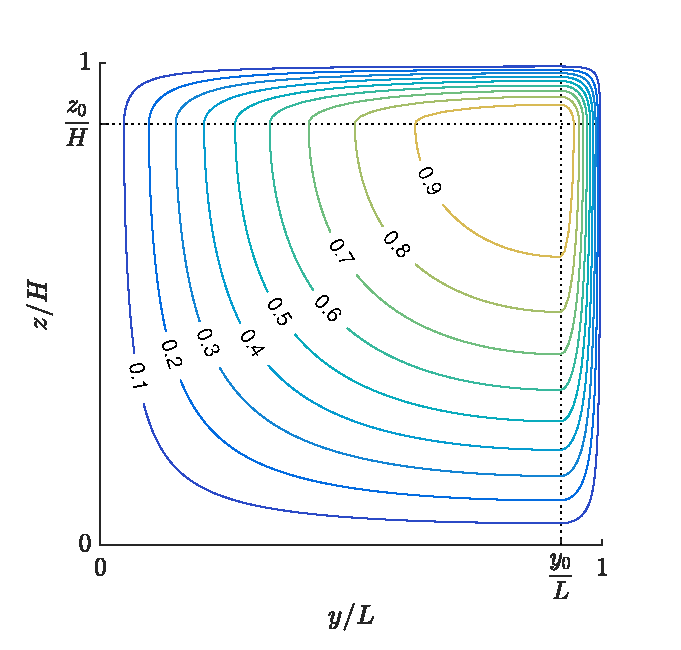
\includegraphics[width=.5\textwidth]{fig/overturner/psi.eps}
	\caption{Some isolines of the adimensional meridian streamfunction $\psi(y,z)/\Psi$, which are also streamlines of the flow.}
	\label{fig:psi_overturner}
\end{figure}

The meridian and vertical components of the velocity are then expressed as
\begin{equation} \label{eq:v_overturner}
	v(y,z) = \Psi\left\{ 
		\begin{array}{lrrr}
			- \phi(y,y_0)\phi'(z,z_0) & \mbox{if} & 0 \le y < y_0, & 0 \le z < z_0,\\
			\phi(y,y_0)\phi'(H-z,H-z_0) & \mbox{if} & 0 \le y < y_0, & z_0 < z \le H,\\
			\phi(L-y,L-y_0)\phi'(H-z,H-z_0) & \mbox{if} & y_0 < y \le L, & z_0 < z \le H,\\
			- \phi(L-y,L-y_0)\phi'(z,z_0) & \mbox{if} & y_0 < y \le L, & 0 \le z < z_0,\\
			- \phi'(z,z_0) & \mbox{if} & y = y_0, & 0 \le z < z_0,\\
			\phi'(H-z,H-z_0) & \mbox{if} & y = y_0, & z_0 < z \le H,\\
			0 & \mbox{if} &0 \le y \le L, & z = z_0.
		\end{array}
	\right.
\end{equation}
and
\begin{equation} \label{eq:w_overturner}
	w(y,z) = \Psi\left\{ 
		\begin{array}{lrrr}
			\phi'(y,y_0)\phi(z,z_0) & \mbox{if} & 0 \le y < y_0, & 0 \le z < z_0,\\
			\phi'(y,y_0)\phi(H-z,H-z_0) & \mbox{if} & 0 \le y < y_0, & z_0 < z \le H,\\
			- \phi'(L-y,L-y_0)\phi(H-z,H-z_0) & \mbox{if} & y_0 < y \le L, & z_0 < z \le H,\\
			- \phi'(L-y,L-y_0)\phi(z,z_0) & \mbox{if} & y_0 < y \le L, & 0 \le z < z_0,\\
			\phi'(y,y_0) & \mbox{if} & 0 \le y < y_0, & 0 \le z = z_0,\\
			- \phi'(L-y,L-y_0) & \mbox{if} & y_0 < y \le L, & z = z_0,\\
			0 & \mbox{if} & y = y_0. &
		\end{array}
	\right.
\end{equation}